
\chapter{Overview of ZMathLang}
\label{ch:design}

Using the methodology of MathLang for mathematics (section \ref{sec:mathlang}), I have created and implemented a step by step way of translating Z specifications into theorem provers with additional checks for correctness along the way. This translation consists of one large framework (executed by a user interface) with many smaller tools to assist the translation. Not only is the translation useful for a novice to translate a Z specification into a theorem prover but it also creates other diagrams and graphs to help with the analysis of a formal system specification.

\begin{figure}[H]
 \begin{center}
 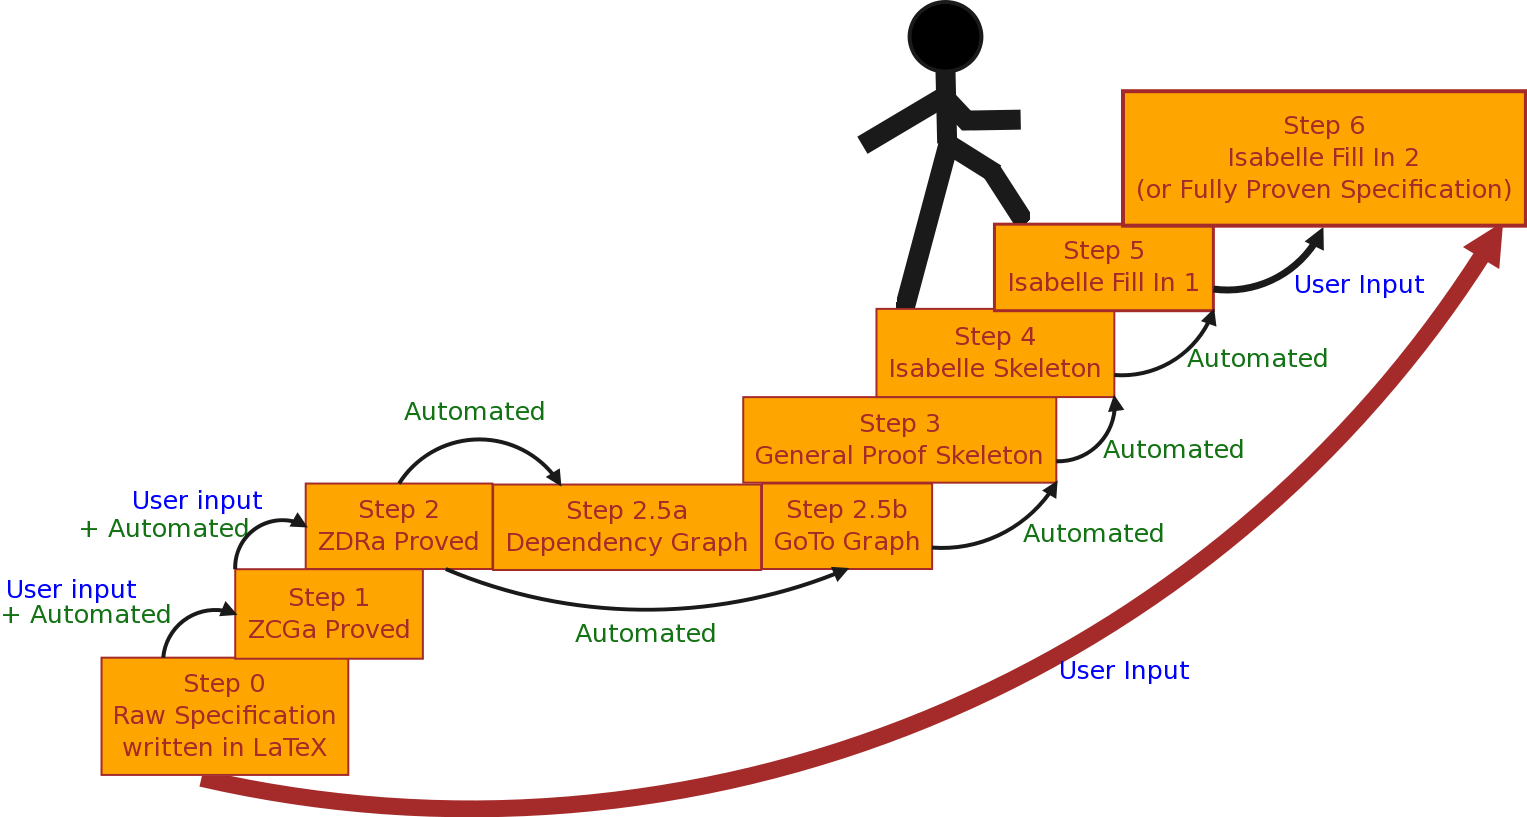
\includegraphics [width=12cm]{Figures/Design/mathlangsteps.png}
 \caption{The steps required to obtain a full proof from a raw specification.}
 \label{fig:steps}
\end{center}
\end{figure} 

The framework is targeted at novices in theorem proving. The users should have some idea of formal specifications but no or little knowledge of the targetted theorem prover. Figure \ref{fig:steps} shows the outline of the framework. The higher the user goes up the steps the more rigorous the checks for correctness. Step 1 and step 2 are interchangable and can be done in any order. However they both must be completed before moving up to step 3. Step 6 is the highest level of rigour and checks for full correctness in a theorem prover. For this thesis I have chose to translate Z specifications into Isabelle, however this framework is an outline for any formal specification into any theorem prover which could done in the future.

The user doesn't need to go all the way to the top to check for correctness, one advantage of breaking up the translation is that the user gets some level of rigour and can be satisfied with some level of correctness along the way. However the main advantage of breaking up the translation is that the level of expertise needed to check for the correctness of a system specification can be done by someone who has little or no expertise in checking for correctness by a theorem prover or otherwise. The small black arrows represent the amount of expertise needed for each step. The last step the arrow is slightly thicker as some theorem prover knowledge is needed. However these arrows are still small in comparison to the red thick arrow which represents the translation in one big step.

The framework breaks the translation into 6 steps most of which are partially or fully automated. These are:

\begin{itemize}
\item Step 0: Raw LaTeX Z Specification. {\color{set}Start}
\item Step 1: Check for Core Grammatical correctness (ZCGa). {\color{set}User Input + Automated}
\item Step 2: Check for Document Rhetorical correctness. {\color{set}(ZDRa) User Input + Automated}
\item Step 3: Generate a General Proof Skeleton (GPSa). {\color{set}Automated}
\item Step 4: Generate an Isabelle Skeleton. {\color{set}Automated}
\item Step 5: Fill in the Isabelle Skeleton. {\color{set}Automated}
\item Step 6: Prove existing lemmas and add more safety properties if needed. {\color{set}User Input}
\end{itemize}

\section{Step 0- The raw LaTeX file}

The first step requires the user to write or have a formal specification they wish to check for correctness. This specification can be fully written in Z or partially written in Z (thus a specification written in english on the way to becoming formalised in Z). The specification should be written in \LaTeX{} format and can be a mix of natural language and Z. An example of a specification written in the Z notation can be seen in figure \ref{fig:zexample}.

\begin{figure}[H]
 \begin{center}
 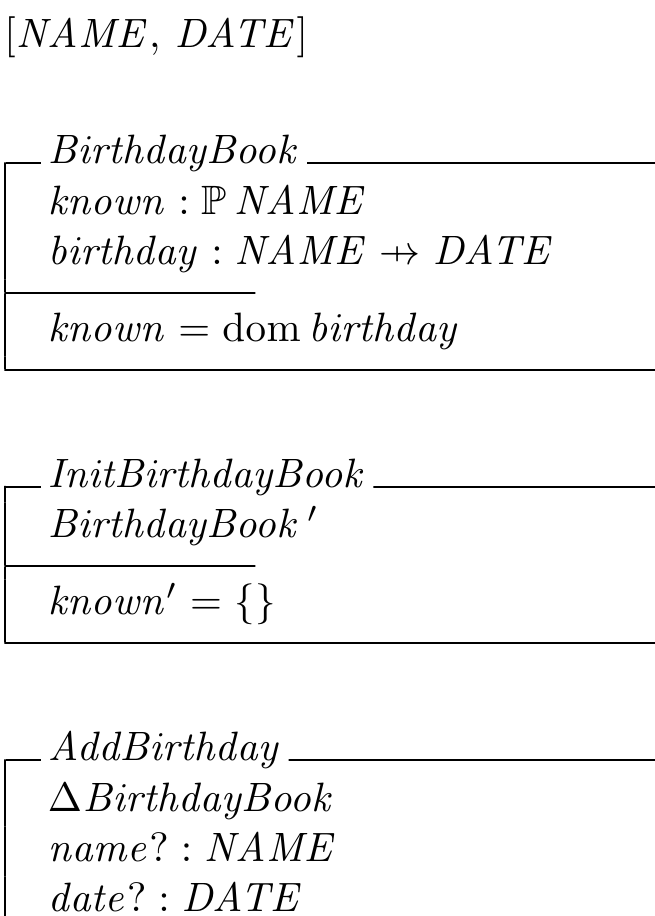
\includegraphics [scale=0.2]{Figures/Design/zspec.png}
 \caption{Example of a partial Z specification.}
 \label{fig:zexample}
\end{center}
\end{figure} 

\section{Step 1- The Core Grammatical aspect for Z}

The next step in figure \ref{fig:steps} shows the specification should be \gls{zcga} proved. Although this step is interchangable with step 2 (\gls{zdra}) it is shown as step 2 on the diagram for convinience. In this step the user annoates their document which they have obtained in step 0 with 7 categories and then checks these for correctness. Figure \ref{fig:steps} show this step is achieved by user input and automation. The user input of this step is the annotations and the automation is the \gls{zcga} checker. This automatically produces a document labeled with the various categories in difference colours and can help identify grammar types to other members interested in the the specification. A \gls{zcga} annotated specification is shown in figure \ref{fig:zcgaexample}. The \gls{zcga} is further explained in chapter \ref{ch:zcga}.

\begin{figure}[H]
 \begin{center}
 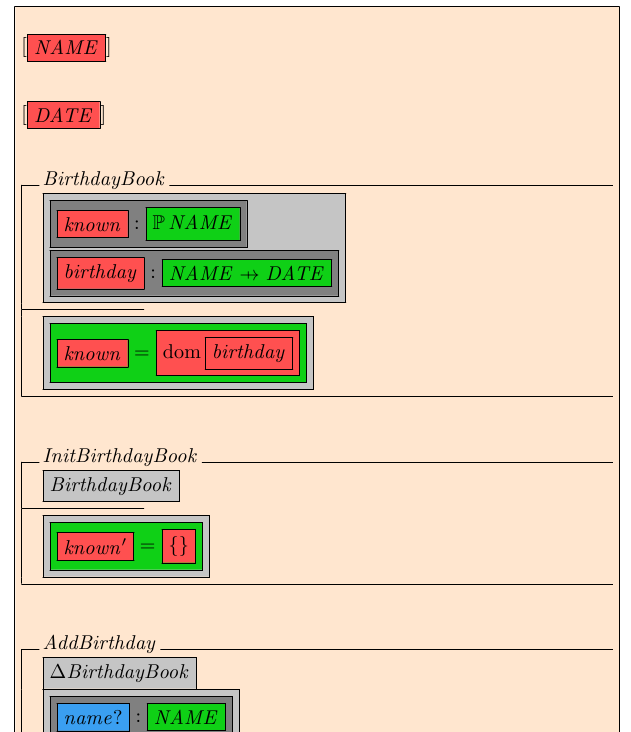
\includegraphics [scale=0.2]{Figures/Design/zcgaexample.png}
 \caption{Example of a ZCGa annotated specification.}
 \label{fig:zcgaexample}
\end{center}
\end{figure} 

\section{Step 2- The document Rhetorical aspect for Z}

The \gls{zdra} (chapter \ref{ch:zdra}) step shown as step 2 in figure \ref{fig:steps} comes before or after the \gls{zcga} step. Similarly to the \gls{zcga} step the user annotates their document from step 0 or step 1 with \gls{zdra} instances and relationships. This chunks parts of the specification and allows the user to describe the relationship between these chunks of specification. The annotation is the user input part of this step and the automation is the \gls{zdra} checker which checks if there are any loops in the reasoning and give warnings if the specification still needs to be totalised. Once the user has annotated this document and compiled it the outputing result shows the specification divided into chunks and arrows showing the relations between the chunks. An example of a Z specification annotated in \gls{zdra} is shown in figure \ref{fig:zdraexample}.

\begin{figure}[H]
 \begin{center}
 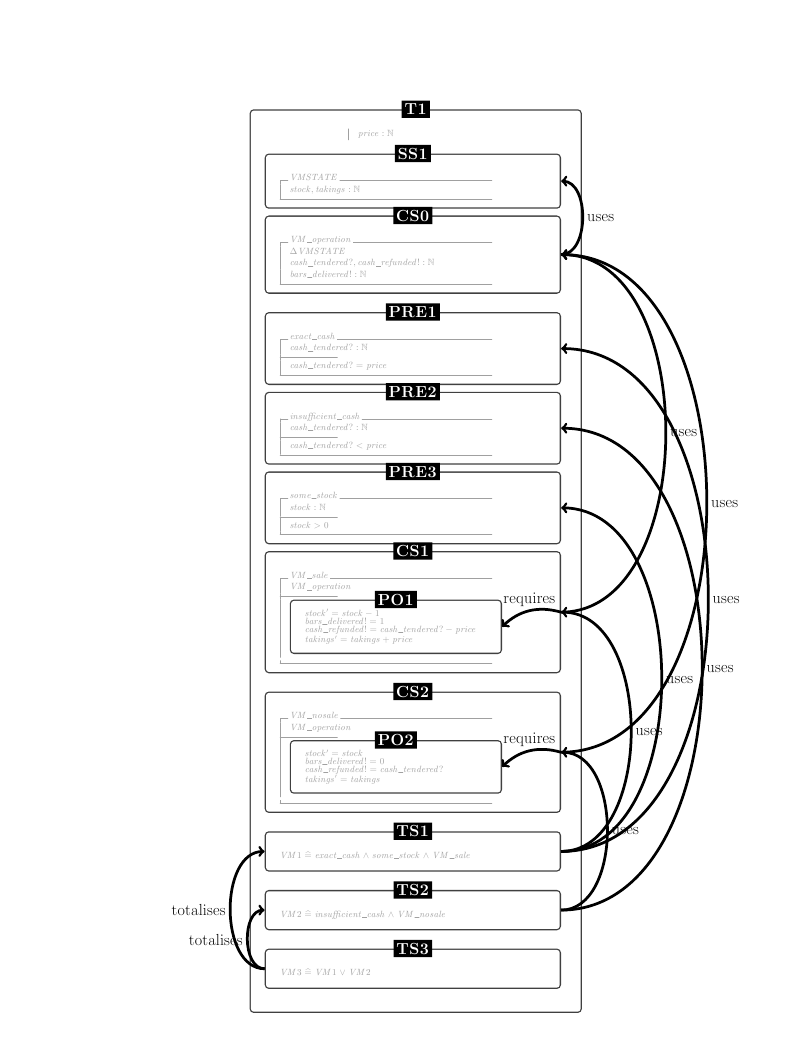
\includegraphics [scale=0.2]{Figures/Design/zdracomp.png}
 \caption{Example of a ZDRa annotated specification.}
 \label{fig:zdraexample}
\end{center}
\end{figure} 

The \gls{zdra} automatically produces a dependency and a goto graph (section \ref{subsec:zdra_prodcuts}), these a shown as 2.5a and 2.5b respectively in figure \ref{fig:steps}. The loops in reasoning are checked in both the dependecy graph and goto graph. An example of a goto graph is shown in figure \ref{fig:gotoexample}.

\begin{figure}[H]
 \begin{center}
 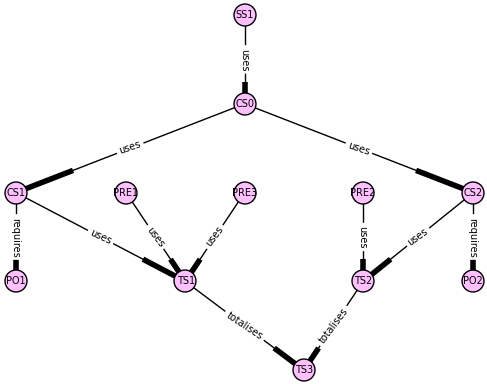
\includegraphics [scale=0.4]{Figures/Design/goto.png}
 \caption{Example of an automatically generated goto graph.}
 \label{fig:gotoexample}
\end{center}
\end{figure} 

\section{Step 3- The General Proof skeleton}

The following step is an automatically generated \gls{gps}. This document is automated using the goto graph which is generated from the \gls{zdra} annotated \LaTeX{} specification. It uses the goto graph to describe in which logical order to input the specification into any theorem prover. At this stage it also adds simple proof obligations to check for the consitancy of the specification i.e. the specification is not conflictive each part. An example of a general proof skeleton is shown in figure \ref{fig:proofskelexample}. The \gls{gps} is further described in section \ref{sec:zdra2gen}.

\begin{figure}[H]
 \begin{center}
 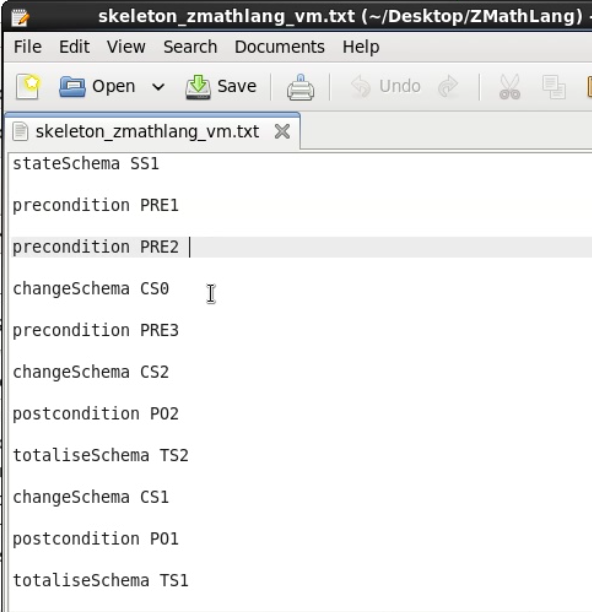
\includegraphics [scale=0.2]{Figures/Design/proofskel.png}
 \caption{Example of a general proof skeleton.}
 \label{fig:proofskelexample}
\end{center}
\end{figure} 

\section{Step 4- The Z specification written as an Isabelle Skeleton}

Using the \gls{gps} in step 3, the instances are then translated into an Isabelle skeleton in step 4. That is the instances of the specification are translated into Isabelle syntax using definitions, lemma's, theorys etc to produce a .thy file. This step is fully automated and thus a user with no Isabelle experience can still get to this stage. An example of a Z specification skeleton written in Isabelle is shown in figure \ref{fig:isaskelexample}. Details of how this translation is conducted is described in section \ref{sec:gpsa2isa} of this thesis.

\begin{figure}[H]
 \begin{center}
 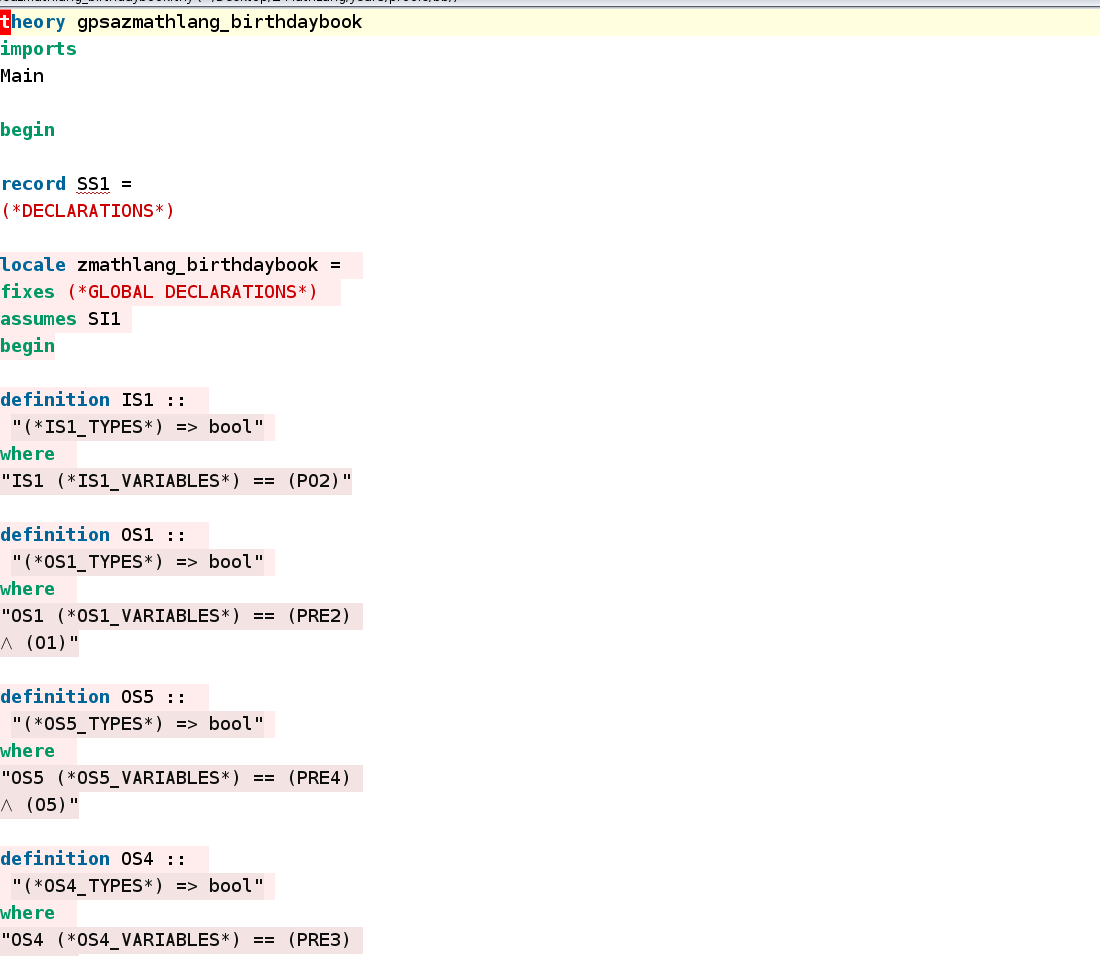
\includegraphics [scale=0.2]{Figures/Design/isaskeleton.png}
 \caption{Example of an Isabelle skeleton.}
 \label{fig:isaskelexample}
\end{center}
\end{figure} 

\section{Step 5- The Z specification written as in Isabelle Syntax}

Step 5 is also automated, using the \gls{zcga} annotated document produced in step 1 and the Isabelle skeleton produced in step 4. This part of the framework fills in the details from the specification using all the declarations, expressions, definition etc in Isabelle syntax. Since the translation can also be done on semi-formal specifications and incomplete formal specification there may be some information missing in the \gls{zcga} such as an expression or a definition. Note the lemmas from the proof obligations created in step 3 will also be filled in, however the actual proofs for these will not and they will be followed by the command `\texttt{sorry}' to artificially complete proofs. An example of a filled in isabelle skeleton is shown in figure \ref{fig:fillin1}.

\begin{figure}[H]
 \begin{center}
 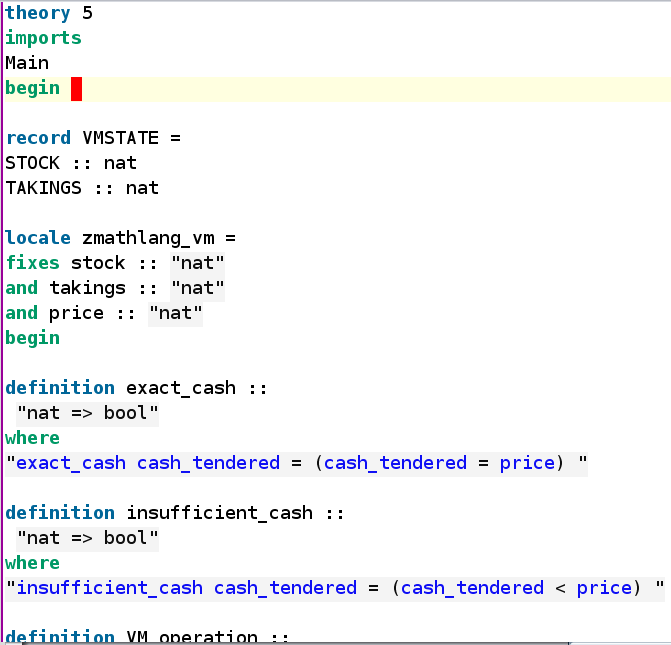
\includegraphics [scale=0.3]{Figures/Design/fillin1.png}
 \caption{Example of an Isabelle skeleton automatically filled in.}
 \label{fig:fillin1}
\end{center}
\end{figure} 

 In this case the Isabelle skeleton will not change. Further information on the translation is described in section \ref{sec:zcga2fillin} of this thesis.

\section{Step 6- A fully proven Z specification}

The final step in the \gls{zmath} framework and the top of the stairs from figure \ref{fig:steps} is to fill in the Isabelle file from step 5. This final step is represented by a slightly thicker arrow in figure \ref{fig:steps} compared with the others as the user may need to have some little theorem prover knowledge to prove properties about the specification. Also if there is some missing information such as missing expressions and definitions the user must fill these out as well in order to have a fully proven specification. However this may be slightly easier then writing the specification from scratch in Isabelle as the user would allready have examples of other instances in their Isabelle syntax form. More details on this last step is described in section \ref{sec:isa2ful} of this thesis.

\section{Procedures and products within ZMathLang}

\begin{figure}[H]
 \begin{center}
 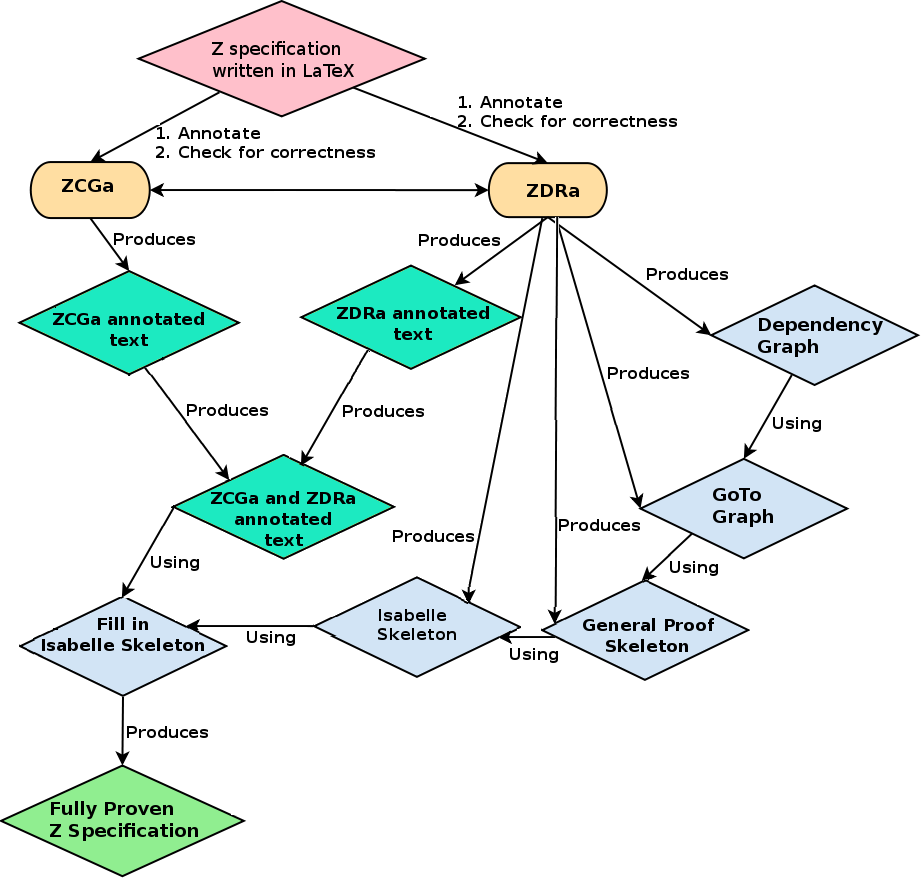
\includegraphics [scale=0.4]{Figures/Design/ZMathLangFlow.png}
 \caption{Flow chart of ZMathLang.}
 \label{fig:zmathflow}
\end{center}
\end{figure} 

Figure \ref{fig:zmathflow} shows a flow chart describing the documents produced from using the framework and which parts are fully automated, partially automated and user input. Products which are created by full automation are diamonds in \colorbox{lightblue}{blue}. Diamonds in \colorbox{lightgreen}{green} are produced by user input and products shown in \colorbox{aqua}{aqua} diamonds are partial automated.

The \colorbox{lightpink}{pink} diamond is the starting point for all users. The \colorbox{lightorange}{orange} ovals describe procedures of the ZCGa and ZDRa. The ZCGa procedure requires user input and automation and produces a `ZCGa annotated text'. The ZDRa procedure requires user input to annotated and the check is automated. Both the \gls{zcga} and \gls{zdra} procedures done together produce a `\gls{zcga} and \gls{zdra} annotated text'. After completing the \gls{zdra} procedure a 'dependency graph' is automatically generated, which can then in turn generate a `GoTo graph' which in turn can create a general proof skeleton. From the `general proof skeleton' we can then create an `Isabelle skeleton'  which can be filled in using information from the `\gls{zcga} and \gls{zdra} annotated text'. Using the `Filled in Isabelle skeleton' the user needs to fill in the missing information to obtain a `fully proven Z specification'.

\section{The ZMathLang LaTeX Package}
\todo[inline]{Describe how the ZMathLang LaTeX package is written}

\subsection{ZCGa part}

\subsection{ZDRa part}

\section{Conclusion}

In total there are 6 steps in order to translate a Z specification into the theorem prover Isabelle. Each of these steps assist the user in understand the specification more, and some steps even produce documents, graphs and charts in order to analyse the specification. These products also allow others in the development team to understand the system better such as clients, stakeholders, developers etc. The majority of the steps are fully automated whilst some a little user input. The next chapter begins to describe step 1 (ZCGa) in more detail.